\documentclass{article}
\title{Blanchard Ch.12}
\author{Dawei Wang}
\date{\today}
\usepackage{ctex}
\usepackage{amsmath}
\usepackage{amssymb}
\usepackage{graphicx} %插入图片的宏包
\usepackage{float} %设置图片浮动位置的宏包
\usepackage{subfigure} %插入多图时用子图显示的宏包
\begin{document}
	\maketitle	

\section{技术进步和增长率}

\subsection{技术进步与生产函数}

技术进步有很多定义:

资本量和劳动力给定,技术进步会提高产出水平。

技术进步会提高产品质量。

技术进步会产生新产品。

技术进步会带来更多样化的产品。

这些定义有很多相似性:消费者在每个情形下都能得到更多服务。如果把产出看作经济体生产产品提供的服务的加总,那么技术进步是在资本和劳动力数量不变的情况下增加产出的因素。把技术因素水平作为一个变量,来判断在资本和劳动力数量给定条件下的产出。用A来表示技术水平,那么生产函数可以表示为:

\[
Y=F(K,N,A)
\]

对上述等式加以约束:

\[
Y=F(K,AN)
\]

这个等式表示产出取决于资本以及劳动力乘以技术水平。

生产同样数量的产出,技术进步减少工人数量。技术水平A翻倍,劳动力数量N减半,
产出水平不变。

工人数量不变,技术进步增加产出。可以把AN看作经济中的有效劳动(effective labor)。技术水平A翻倍,就相当于经济中劳动力的数量翻倍。也就是说,产出由两个因素得来:资本K和有效劳动AN。

AN有时也叫以效率为单位的劳动(labor in efficiency units)。

单位有效工人:除以有效劳动的数量AN。

\hspace*{\fill}

对生产函数的约束:

假设依然存在规模经济不变:

\[
xY=F(xK,xAN)
\]

假设资本和劳动力两个因素都存在规模报酬递减。

\[
\frac{Y}{AN}=F(\frac{K}{AN},1)
\]

定义函数式f,$ f(\frac{K}{AN})=F(\frac{K}{AN},1) $:

\[
\frac{Y}{AN}=f(\frac{K}{AN})
\]

\begin{figure}[H] %H为当前位置,!htb为忽略美学标准,htbp为浮动图形
	\centering %图片居中
	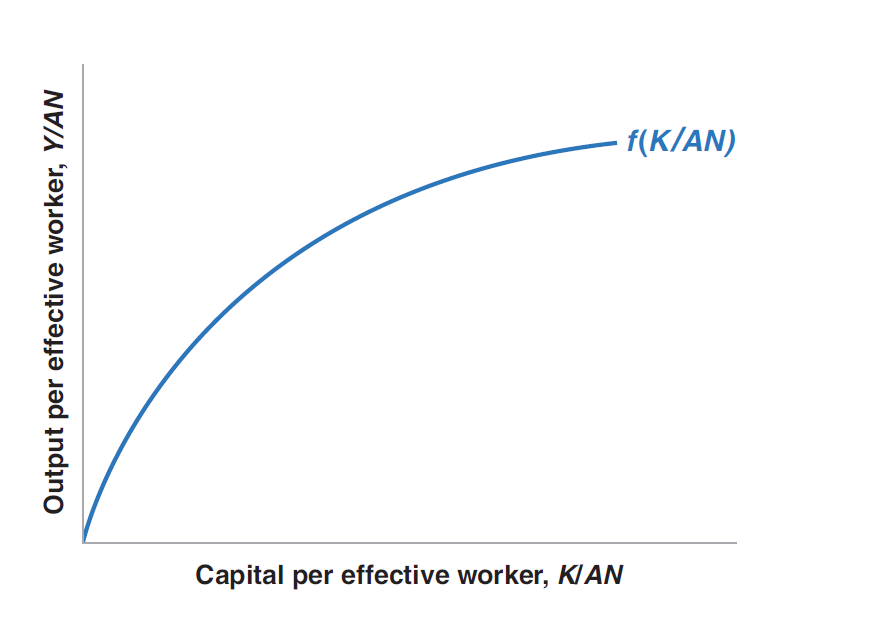
\includegraphics[width=1\textwidth]{12_1} %插入图片,[]中设置图片大小,{}中是图片文件名
	\caption{Output per Effective
		Worker versus Capital per
		Effective Worker} %最终文档中希望显示的图片标题
	\label{Fig.main2} %用于文内引用的标签
\end{figure}

总结:单位有效工人的产出是单位有效工人资本的函数

\subsection{产出和资本的关系}

人均资本在长期中是增加还是减少,取决于人均投资比人均折旧大还是小。人均产出也是如此。

\begin{figure}[H] %H为当前位置,!htb为忽略美学标准,htbp为浮动图形
	\centering %图片居中
	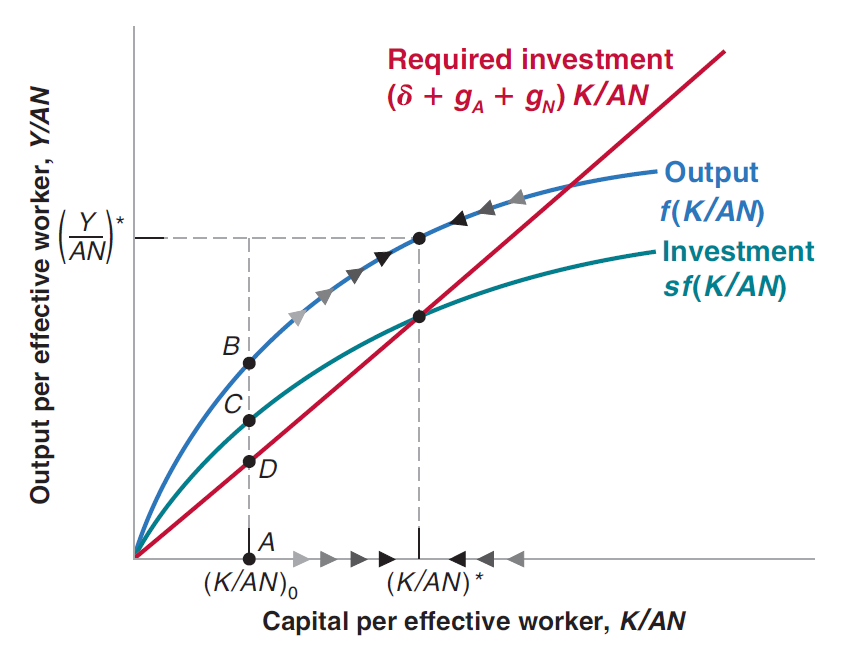
\includegraphics[width=1\textwidth]{12_2} %插入图片,[]中设置图片大小,{}中是图片文件名
	\caption{The Dynamics of Capital
		per Effective Worker
		and Output per Effective
		Worker} %最终文档中希望显示的图片标题
	\label{Fig.main3} %用于文内引用的标签
\end{figure}

单位有效工人产出随单位有效工人资本的增加而增加,但增加速率下降。

假设投资等于私人储蓄,私人储蓄是固定的,则投资为:

\[
I=S=sY
\]

等式两边除以有效劳动的数量AN,得:

\[
\frac{I}{AN}=s\frac{Y}{AN}
\]

\[
\frac{I}{AN}=sf(\frac{K}{AN})
\]

设定$\delta$为资本折旧率,技术进步率为$ g_A $,人口增长率为$ g_N $。假定就业人数与总人口的比例保持不变,则劳动力数量以$ g_N $的速度增长。由此可得,有效劳动的增长率为($ g_A+g_N $)。

保持单位有效劳动的资本存量水平不变的投资为:

\[
I=\delta K+(g_A+g_N)K
\]

即:

\[
I=(\delta+g_A+g_N)K
\]

$\delta K$是为了保持资本存量不变,额外的资本$ (g_A+g_N)K $是为了确保资本存量和有效劳动数量的增长保持一致。

等式两边同时除以有效劳动的数量,得出保持单位有效工人的资本存量水平不变的单位有效工人投资量为:

\[
\frac{I}{AN}=(\delta+g_A+g_N)\frac{K}{AN}
\]

上图中向上倾斜的“必要投资”曲线是使单位有效工人的资本存量水平不变的单位有效工人的投资量,其斜率为($ \delta+g_A+g_N $)。

\subsection{资本和产出的动态变化}

长期中,单位有效工人资本达到稳定水平,单位有效工人产出也达到稳定水平。也就是说,稳态经济中单位有效工人和单位有效工人产出分别为$ (K/AN)^* $、$ (Y/AN)^* $。

这意味着在稳态经济中,产出Y和有效劳动AN的增长速度是一样的。有效劳动的增长率为$ (g_A+g_N) $,所以稳态下的产出增长率也为$ g_A+g_N $。资本存量也一样,即稳态下单位有效工人的资本存量是不变的,其增长率也为$ (g_A+g_N) $。

稳态经济中,产出增长率等于人口增长率$ g_N $加技术进步率$ g_A $,这也表明产出增长率与储蓄率无关。

有效劳动的数量以$ (g_A+g_N) $的速率增长,若经济的产出增长率超过$ (g_A+g_N) $,由于资本的规模报酬递减,因此资本的增长速度需要快于产出。产出中用于资本积累的部分越来越多,在某一点,不可能有多余产出。因此,经济的增长速度不可能永远快于$ (g_A+g_N) $。

由于产出增长率为$ (g_A+g_N) $,工人数量的增长率为$ g_N $,因此人均产出的增长率为$ g_A $。也就是说,在稳态经济中,人均产出的增长率等于技术进步率。

由于稳态下的产出、资本和有效劳动的增长速度都为$ (g_A+g_N) $,因此这种稳态下的经济称为均衡增长(balanced growth)。在稳态经济中,产出、资本和有效劳动两种投入要素以同样的速率均衡增长。

\begin{figure}[H] %H为当前位置,!htb为忽略美学标准,htbp为浮动图形
	\centering %图片居中
	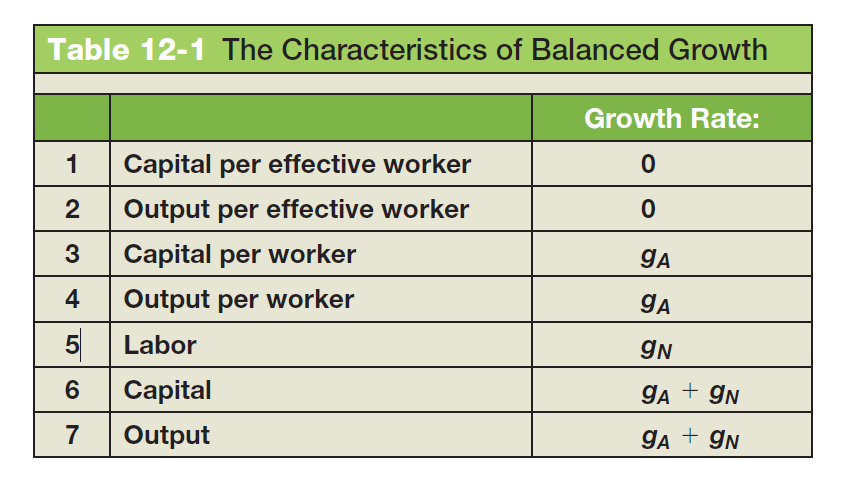
\includegraphics[width=1\textwidth]{12_3} %插入图片,[]中设置图片大小,{}中是图片文件名
	%\caption{} %最终文档中希望显示的图片标题
	\label{Fig.main4} %用于文内引用的标签
\end{figure}

\subsection{储蓄率的影响}

储蓄率对稳态经济的的增长率没有影响,但是储蓄率的提高会提高单位有效工人的产出水平。

\begin{figure}[H] %H为当前位置,!htb为忽略美学标准,htbp为浮动图形
	\centering %图片居中
	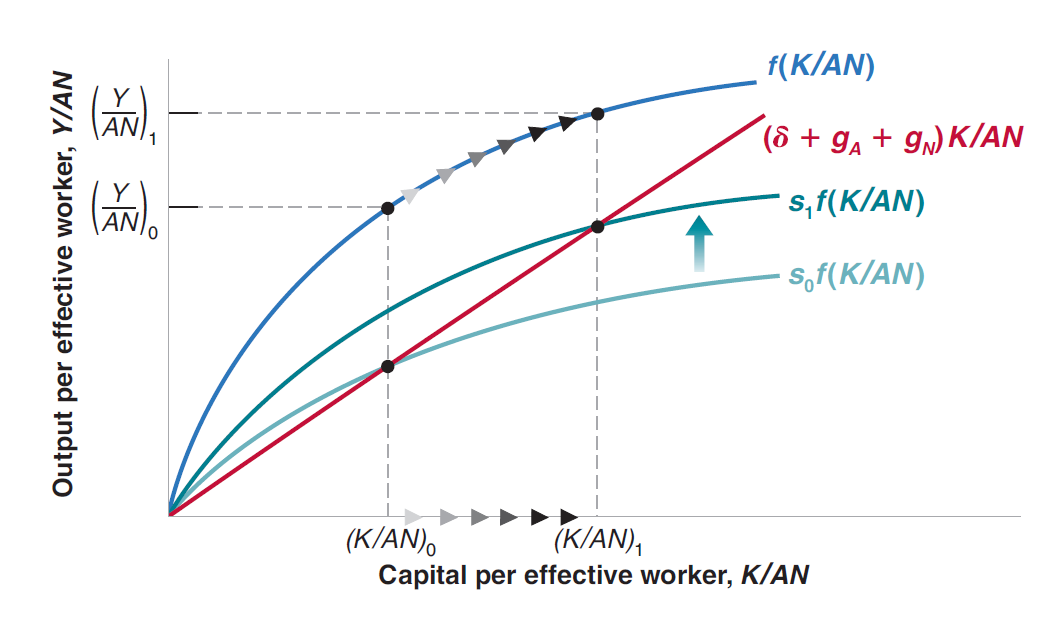
\includegraphics[width=1\textwidth]{12_4} %插入图片,[]中设置图片大小,{}中是图片文件名
	\caption{The Effects of an Increase
		in the Saving Rate: I} %最终文档中希望显示的图片标题
	\label{Fig.main5} %用于文内引用的标签
\end{figure}

\begin{figure}[H] %H为当前位置,!htb为忽略美学标准,htbp为浮动图形
	\centering %图片居中
	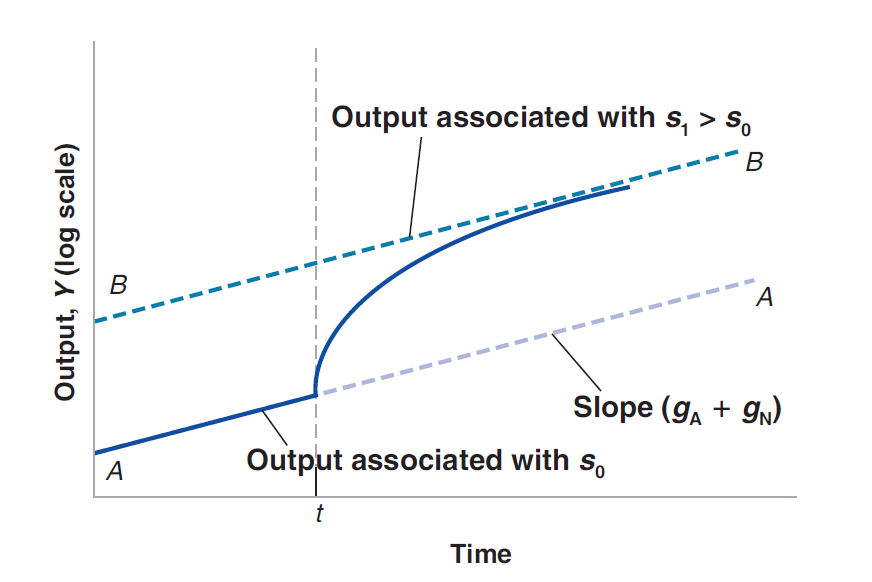
\includegraphics[width=1\textwidth]{12_5} %插入图片,[]中设置图片大小,{}中是图片文件名
	\caption{The Effects of an Increase
		in the Saving Rate: II} %最终文档中希望显示的图片标题
	\label{Fig.main6} %用于文内引用的标签
\end{figure}

经济最初处在均衡增长路径AA,产出的增长率为$ (g_A+g_N) $,故AA曲线的斜率为$ (g_A+g_N) $。在t时储蓄率提高后,产出在一定时间里加快,最终,产出达到比没有储蓄率增加的产出更高的水平,但增长率仍为$ (g_A+g_N) $,即在新的稳态下,经济增长率不变,但处于更高的增长路径BB上。BB线和AA线平行,斜率也为$ (g_A+g_N) $。

稳态下的产出增长率和储蓄率无关,但储蓄率影响稳态下的单位有效工人的产出水平,储蓄率提高后,在一段时间内会使经济增长率超过稳态下的增长率。

\section{技术进步下的决定因素}

现代经济的大多数技术进步是一个很单一的过程,来自企业研发(research and development, R\&D)的结果。

事实上,研发的结果往往是概念,和机器不同,这些概念能被很多企业同时使用。企业购置新机器后,不必担心这个机器被其他企业使用。成功研发产品的企业则没有这些假定。

研发支出水平不仅取决于研究的多产性(fertility of research)——研发支出如何转化为新概念和新产品,还取决于研究成果的专属性(appropriablility)——企业能在多大程度上从研发成果获得利益。

\subsection{研究的多产性}

研究的多产性取决于基础研究和应用研发的良好互动。基础研究本身不能带来技术进步,但成功的应用研发最终取决于基础研究。

重要发明的全部潜在价值往往需要很多年,甚至上百年才能发掘出来。一般的顺序是,重要的发明带来新的潜在实际运用,然后出现新的产品,这些新产品最终得以推广运用。

\subsection{研究成果的专属性}

更重要的因素是新产品的法律保护。没有法律保护的话,企业从研发新产品中得到的利润会很少。专利(patent)赋予了研制新产品的企业在特定时间内不允许其他企业使用该新产品的权利。

政府制定专利法一方面要对新产品进行保护使企业有动力去投入研发;另一方面,企业一旦研制出新产品,当其他企业和人们能自由使用这些新产品的相关知识和技术时,最有益于社会。因此专利法的制定需要权衡。

\section{制度、技术进步和增长}

经济学家认为,产权的保护可能是最重要的。如果人们预期赚得的利润会被政府侵吞,或者行贿给腐败官僚,或者被其他人盗取,那么就没有人愿意去创办企业,引进新技术以及投资于研发。

产权保护实际上意味着完善的政治体制,当局者不能剥夺公民财产;意味着完善的司法体系,能迅速有效解决不平等。


\section{增长的事实:重新观察}

假定一国经济中,人均产出在一段时间内呈现高增长。理论表明这种高增长可能来自两方面:

可能反映了均衡增长下的高技术进步率;

也可能反映了单位有效工人的资本存量$ K/AN $增加。单位有效工人的资本存量会带来一定时期的高增长,即便技术进步率保持不变。

如果高增长反映高均衡增长,那么人均产出的增长率等于技术进步率。如果高增长反映单位有效工人的资本存量$ K/AN $向更高水平调整,那么调整的幅度就是人均产出增长率超过技术进步率的部分。

资本积累使一个国家的产出对资本的比例保持不变,从而维持均衡增长。这就是说,在一段时间内,经济增长并非来自资本积累的显著增长。

\section{怎样衡量技术进步}




































































	
\end{document}